\subsubsection{Spherical Coordinate}

\begin{tabular}{ccc}
{$\begin{aligned}
  x = r\sin\theta\cos\phi \\
  y = r\sin\theta\sin\phi \\
  z = r\cos\theta
\end{aligned}$}
&
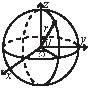
\includegraphics[width=25mm]{../codes/Misc/sphericalCoordinates.pdf}
&
{$\begin{aligned}
  r = \sqrt{x^2+y^2+z^2} \\
  \theta = \textrm{acos}(z/\sqrt{x^2+y^2+z^2}) \\
  \phi = \textrm{atan2}(y,x)
\end{aligned}$}
\end{tabular}

\subsubsection{Sherman-Morrison formula}
$\left(A + uv^\textsf{T}\right)^{-1} = A^{-1} - \frac{A^{-1}uv^\textsf{T}A^{-1}}{1 + v^\textsf{T}A^{-1}u}$

\subsubsection{Kirchhoff's Theorem}
Denote $L$ be a $n \times n$ matrix as the Laplacian matrix of graph $G$, where $L_{ii} = d(i)$, $L_{ij} = -c$ where $c$ is the number of edge $(i, j)$ in $G$.
\begin{itemize}[nosep]
    \item The number of undirected spanning in $G$ is $\det(\tilde{L}_{11})$.
    \item The number of directed spanning tree rooted at $r$ in $G$ is $\det(\tilde{L}_{rr})$.
\end{itemize}

\subsubsection{Random Walk on Graph}
Let $P$ be the transition matrix of a strongly connected directed graph, $\sum _ j P_{i,j} = 1$.
Let $F_{i,j}$ be the expected time to reach $j$ from $i$.
Let $g_i$ be the expected time from $i$ to $i$, $G = \operatorname{diag}(g)$
and $J$ be a matrix all of 1, i.e. $J_{i,j} = 1$.
Then, $F = J - G + PF$

First solve $G$: let $\pi P = \pi$ be a stationary distribution. Then $\pi_i g_i = 1$.
The rank of $I - P$ is $n - 1$, so we first solve a special solution $X$ such that $(I - P)X = J - G$ and adjust $X$ to $F$ by
$F_{i,j} = X_{i,j} - X_{j,j}$.

\subsubsection{Tutte's Matrix}
Let $D$ be a $n \times n$ matrix, where $d_{ij} = x_{ij}$ ($x_{ij}$ is chosen uniform randomly) if $i < j$ and $(i, j) \in E$, otherwise $d_{ij} = -d_{ji}$. $\frac{rank(D)}{2}$ is the maximum matching on $G$.

\subsubsection{Cayley's Formula}
\begin{itemize}[nosep]
  \item Given a degree sequence $d_1, d_2, \ldots, d_n$ for each labeled vertices, there're $\frac{(n - 2)!}{(d_1 - 1)!(d_2 - 1)!\cdots(d_n - 1)!}$ spanning trees.
  \item Let $T_{n, k}$ be the number of labeled forests on $n$ vertices with $k$ components, such that vertex $1, 2, \ldots, k$ belong to different components. Then $T_{n, k} = kn^{n - k - 1}$.
\end{itemize}

\subsubsection{Erdős–Gallai theorem}
A sequence of non-negative integers $d_1 \geq d_2 \geq \ldots \geq d_n$ can be represented as the degree sequence of a finite simple graph on $n$ vertices if and only if $d_1 + d_2 + \ldots + d_n$ is even and
$$ \sum_{i = 1}^{k}d_i \leq k(k - 1) + \sum_{i = k + 1}^{n}\min(d_i, k) $$
holds for all $1 \leq k \leq n$.

\subsubsection{Havel–Hakimi algorithm}
find the vertex who has greatest degree unused, connect it with other greatest vertex.

\subsubsection{Gale–Ryser theorem}
A pair of sequences of nonnegative integers $a_1\ge\cdots\ge a_n$ and $b_1,\ldots,b_n$ is bigraphic if and only if $\displaystyle\sum_{i=1}^n a_i=\displaystyle\sum_{i=1}^n b_i$ and $\displaystyle\sum_{i=1}^k a_i\le \displaystyle\sum_{i=1}^n\min(b_i,k)$ holds for every $1\le k\le n$.

\subsubsection{Fulkerson–Chen–Anstee theorem}
A sequence $(a_1,b_1),\ldots,(a_n,b_n)$ of nonnegative integer pairs with $a_1\ge\cdots\ge a_n$ is digraphic if and only if $\displaystyle\sum_{i=1}^n a_i=\displaystyle\sum_{i=1}^n b_i$ and $\displaystyle\sum_{i=1}^k a_i\le \displaystyle\sum_{i=1}^k\min(b_i,k-1)+\displaystyle\sum_{i=k+1}^n\min(b_i,k)$ holds for every $1\le k\le n$.

%\subsubsection{Hall's marriage theorem}
%Let $G$ be a finite bipartite graph with bipartite sets $X$ and $Y$.
%For a subset $W$ of $X$, let $N_G(W)$ denote the set of all vertices in $Y$ adjacent to some element of $W$. Then there is an $X$-saturating matching iff $\forall W \subseteq X, |W| \leq |N_G(W)|$

\subsubsection{Euler's planar graph formula}
$V-E+F=C+1$. $E\leq 3V-6$ (when $V\geq 3$)

\subsubsection{Pick's theorem}
For simple polygon, when points are all integer, we have $A=\text{\#\{lattice points in the interior\}} + \frac{\text{\#\{lattice points on the boundary\}}}{2} - 1$

%\subsubsection{Lucas's theorem}
%$\binom{m}{n}\equiv\prod_{i=0}^k\binom{m_i}{n_i}\pmod p$, where $m=m_kp^k+m_{k-1}p^{k-1}+\cdots +m_1p+m_0$, and $n=n_kp^k+n_{k-1}p^{k-1}+\cdots +n_1p+n_0$.

\subsubsection{Matroid Intersection}
Given matroids \(M_1=(G,I_1),M_2=(G,I_2)\), find maximum \(S\in I_1\cap I_2\).
For each iteration, build the directed graph and find a shortest path from \(s\) to \(t\).
\begin{itemize}[nosep]
    \item \(s \to x: S \sqcup \{x\} \in I_1\)
    \item \(x \to t: S \sqcup \{x\} \in I_2\)
    \item \(y \to x: S \setminus \{y\} \sqcup \{x\} \in I_1\) (\(y\) is in the unique circuit of \(S \sqcup \{x\}\))
    \item \(x \to y: S \setminus \{y\} \sqcup \{x\} \in I_2\) (\(y\) is in the unique circuit of \(S \sqcup \{x\}\))
\end{itemize}
Alternate the path, and \(|S|\) will increase by \(1\).
Let \(R = \min(\operatorname{rank}(I_1), \operatorname{rank}(I_2)), N = |G|\).
In each iteration, \(|E| = O(RN)\).
For weighted case, assign weight \(-w(x)\) and \(w(x)\) to \(x\in S\) and \(x\notin S\), resp.
Use Bellman-Ford to find the weighted shortest path.
The maximum iteration of Bellman-Ford is \(2R+1\).

\subsubsection{Dual of LP}

\begin{tabular}{|l|l|}
\hline
\textbf{Primal} & \textbf{Dual} \\
\hline
Maximize $c^\intercal x$ s.t. $Ax \leq b$, $x \geq 0$ & Minimize $b^\intercal y$ s.t. $A^\intercal y \geq c$, $y \geq 0$ \\
\hline
Maximize $c^\intercal x$ s.t. $Ax \leq b$ & Minimize $b^\intercal y$ s.t. $A^\intercal y = c$, $y \geq 0$ \\
\hline
Maximize $c^\intercal x$ s.t. $Ax = b$, $x \geq 0$ & Minimize $b^\intercal y$ s.t. $A^\intercal y \geq c$ \\
\hline
\end{tabular}

\subsubsection{Parallel Axis Theorem}
The second moment of area $I_z = \int\int x^2+y^2 \mathrm{d}A$
$I_{z'} = I_z + Ad^2$ where $d$ is the distance between two parallel axis $z, z'$.
